\section{Execution}

% \begin{wrapfigure}{R}{0.3\textwidth}
	% \centering
	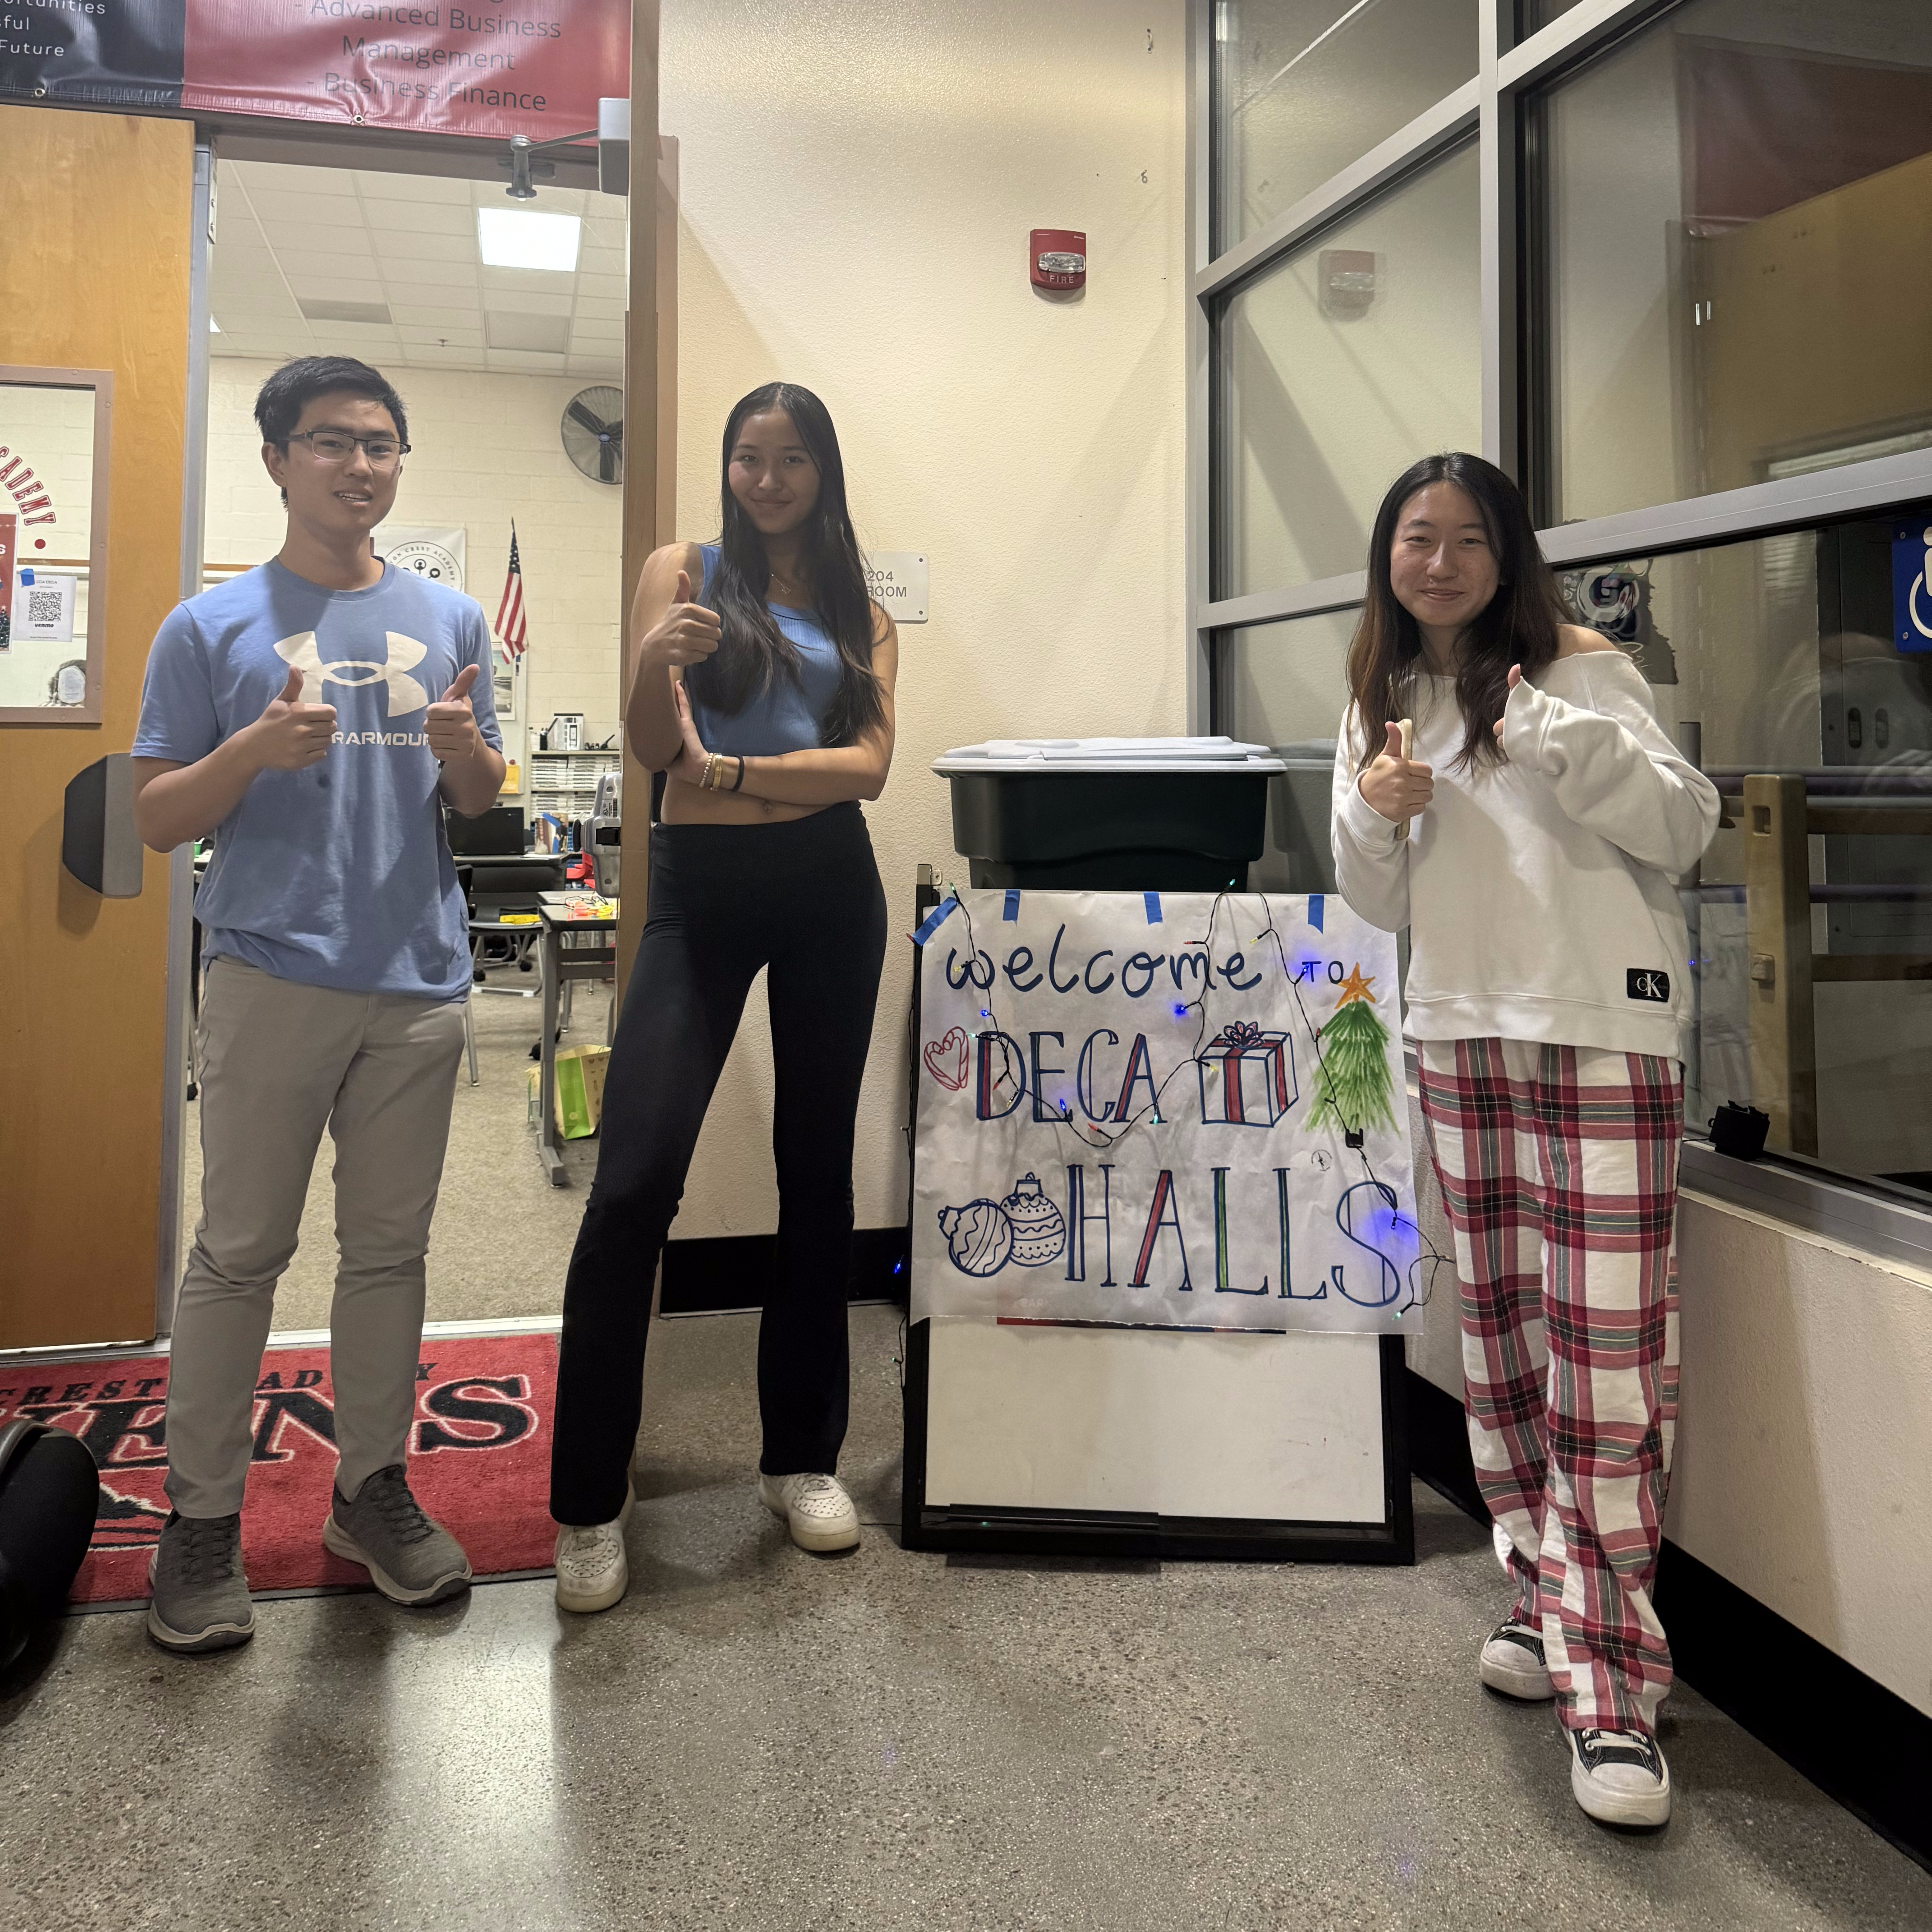
\includegraphics[width=0.28\textwidth]{group.png}
	% \caption{(from left to right) Nathan Dai, Ruby Gao, Lynn Huang}
% \end{wrapfigure}

Our DECA chapter embarked on a fundraising journey with an initial capital of \$210, generously donated by parents through our GoFundMe campaign. We organized a carnival, which, despite a lower-than-expected turnout from AP Statistics students, was a success. The carnival featured a variety of games, including Nerd Nerf Battle Turf, Wheel of Fortune, Chess vs. Wayne, Las Vegas Casino, Steven the Dinosaur, Chopsticks vs. Asian Dad, Tip Jar, and Papa's Ramenria. Detailed rules and a comprehensive list of these games can be found in Appendix \ref{appendix:carnival_games}.

In addition to the games, we also offered hot chocolate and Christmas-themed goodie bags for sale. The carnival raised \$172. Subsequently, we sold our remaining prizes at the Swap Meet and other venues, generating an additional \$205.

We also hosted several food-related fundraisers. Our partnership with Happy Lemon and Chipotle, where a portion of the proceeds from flyer-presenting customers was donated to DECA, resulted in earnings of \$25 and \$71, respectively. On-campus food truck events with Kona Ice and Wetzel Pretzel right after school contributed \$50 and \$165, respectively, to our funds.

